\documentclass[12pt,a4paper]{article}
\usepackage[utf8]{inputenc}
\usepackage[czech]{babel}
\usepackage[T1]{fontenc}
\setlength{\parskip}{6pt}
\usepackage{ amssymb }
\usepackage{ mathrsfs }
\usepackage{amsthm}
\usepackage{amsmath}
\usepackage{fixltx2e}
\newtheorem{definition}{Definice}
\newtheorem{sentence}{Věta}
\newtheorem{example}{Příklad}
\usepackage{graphicx}
\usepackage{ dsfont }

\begin{document}

\title{Státnicový okruh 1: \\ Matematické metody}
\maketitle
\newpage
\tableofcontents
\newpage
\textbf{Množiny, operace s množinami, kartézský součin množin, konečné, spočetné a nespočetné množiny. Číselné
množiny. Princip indukce. Relace a jejich vlastnosti, operace s relacemi, reprezentace relací. Binární relace na
množině, uzávěry relací, ekvivalence, rozklad na množině, uspořádané množiny. Zobrazení a jejich vlastnosti.}

\section{Množiny}
Množina je objekt, který se skládá z jiných objektů tzv. \textbf{prvků} té množiny. Množiny zpravidla značíme velkými písmeny (A, B, \dots, Z), jejich prvky pak malými písmeny (a, b, \dots, z). Fakt, že $x$ je prvkem množiny $A$ značíme $x \in A$. Není-li prvkem $A$ značíme $x \not\in A$.

Množina je jednoznačné dána svými prvky. Prvek do množiny buď patní nebo ne. Nemá tedy smysl hovořit o pořadí prvků a také nemá smysl zabývat se tím kolikrát se daný prvek v množině nachází.
Speciální množinou je tzv. \textbf{prázdná množina} značíme $\emptyset$. Tato množina neobsahuje žádné prvky tedy pro všechna $x$ platí, že $x \not\in \emptyset$.

\subsection{Dělení množin}
Množiny dělíme na \textbf{konečné} a \textbf{nekonečné}. Množina $A$ se nazývá konečná právě když existuje přirozené číslo $n$ tak že prvky této množiny můžeme očíslovat čísly 1, 2, \dots, $n$. Číslo $n$ nazveme počet prvků množiny a značíme jej $|A|$
Pokud $|A| = \infty$ nazveme množinu nekonečnou a říkáme, že má nekonečně mnoho prvků.

\textbf{Spočetná} množina znamená zjednodušeně řečeno „množina, jejíž prvky lze spočítat“. Spočítáním se zde rozumí očíslování prvků množiny přirozenými čísly - přitom je jedno, zda použiji konečný nebo nekonečný počet přirozených čísel.

\subsection{Zapisování množin}
Množiny můžeme zapisovat následujícími způsoby:
\begin{enumerate}
	\item \textbf{Výčtem prvků} - Množinu která obsahuje prvky $a_1,a_2,\dots,a_n$ zapíšeme následovně $\{a_1,a_2,\dots,a_n\}$.
	\item \textbf{Pomocí charakteristické vlastnosti} - Množina obsahuje právě ty prvky, které splňují vlastnost $\varphi(x)$ zapisujeme $\{x | \varphi(x)\}$. Vlastnost $\varphi(x)$ může být popsána i slovně. Příklad $\varphi(x)$: číslo x je sudé.
\end{enumerate}
\subsection{Vztahy mezi množinami}
Základními vztahy mezi množinami jsou \textbf{rovnost} (=) a \textbf{inkluze} ($\subseteq$)
\begin{itemize}
	\item[] $A = B$ znamená, že pro každé $x : x \in A$ právě když $x \in B$
	\item[] $A \subseteq B$ znamená, že pro každé $x$ : jestliže $x \in A$ pak $x \in B$
	\item[] $A \not= B$ znamená že neplatí $A = B$
	\item[] $A \not\subseteq B$ znamená, že neplatí $A \subseteq B$
\end{itemize}

Množina jejichž prvky jsou právě všechny podmnožiny dané množiny $X$, nazýváme \textbf{potenční množina} množiny $X$ značí se $\mathscr{P}(X)$ nebo také $2^X$. Tedy $2^X = \{A|A\subseteq X\}$.

\subsection{Operace s množinami}
Mezi základní operace s množinami patří průnik (značí se $\cap$), sjednocení (značí se $\cup$), rozdíl (značí se $\setminus$).

Jsou-li $A,B$ množiny, definujeme množiny $A \cup B, A \cap B, A \setminus B$ následovně:
\begin{itemize}
	\item[] $A \cap B = \{ x|x \in A \text{ a } x \in B\}$ 
	\item[] $A \cup B = \{ x|x \in A \text{ nebo } x \in B\}$ 
	\item[] $A \setminus B = \{ x|x \in A \text{ a } x \not\in B\}$ 
\end{itemize}

Množiny nazýváme navzájem disjunktní právě když $A \cap B = \emptyset$.

\subsubsection{Vlastnosti operací}
\begin{itemize}
	\item $A \cap \emptyset = \emptyset, \hspace{10pt} A \cup \emptyset = A,\hspace{10pt} A \cap A = A$
	\item $A \cup B = B \cup A, \hspace{10pt} A \cap B = B \cap A$
	\item $(A \cup B) \cup C = A \cup (B \cup C)$
	\item $A \cap (B \cup C) = (A \cap B) \cup (A \cap C), \hspace{10pt} A \cup (B \cap C) = (A \cup B) \cap (A \cup C)$ 
	\item $A \cup (A \cap B) = A, \hspace{10pt} A \cap (A \cup B) = A$ 
\end{itemize}

\section{Relace}
Pojem relace je matematickým protějškem pojmu \textit{vztah}. Různé objekty jsou nebo nejsou v různých vztazích. Například číslo 3 je ve vztahu \uv{být menší} s číslem 5. Vztah je také určen aritou tj. počtem objektů které do vztahu vstupují, výše uvedený příklad má aritu 2 protože porovnáváme 2 čísla. Takovou relaci nazveme binární. Dále máme unární (jeden prvek), ternární (tři prvky), \dots

\begin{definition}
Kartézský součin množin $X_1, X_2, \dots,X_n$ je množina $X_1 \times X_2 \times \dots \times X_n$ definovaná předpisem $$X_1 \times \dots \times X_n =  \{\langle x_1, \dots x_n \rangle | x_1 \in X_1, \dots, x_n \in X_n\} $$
\end{definition}
 Kartézský součin $n$ množin je množina všech uspořádaných n-tic prvků z těchto množin. Je-li $X_1 = \dots = X_n = X$ pak $X_1 \times \dots \times X_n$ značíme také $X^n$ (n-tá kartézská mocnina množiny $X$)

\begin{definition}
Nechť $X_1, \dots,X_n$ jsou množiny. Relace mezi $X_1, \dots,X_n$ je libovolná podmnožina kartézského součinu $X_1 \times \dots \times X_n $.
\end{definition}

\begin{example}
Mějme množinu $A = \{1,2,3,4\}$ a množinu $B = \{a,b,c,d\}$. Relace $R,S \subseteq A \times B$ mohou vypadat následovně. $$R = \{\langle 1, a\rangle, \langle 1, b\rangle, \langle 3, d\rangle, \langle 4, a\rangle\}$$
$$S = \{\langle 3, a\rangle, \langle 1, c\rangle,  \langle 4, c\rangle\}\}$$
\end{example}

\subsection{Operace s (binárními) relacemi}
Relace jsou množiny n-tic. Proto s nimi jde provádět množinové operace ($\cap,\cup,\setminus$) a lze na ně aplikovat rovnost a inkluzi ($=, \subseteq$).
S binárními relacemi můžeme provádět další operace. Začněme tzv. inverzní relací k relaci $R \subseteq X \times Y$ je relace $R^{-1}$ definovaná předpisem: $$R^{-1} = \{\langle y, x \rangle | \langle x, y \rangle \in R\}$$
Další operací je tzv. skládání Je-li $R$ relací mezi množinami $X$ a $Y$ a $S$ relací mezi množinami $Y$ a $Z$, pak složením relací $R$ a $S$ je relace \( R \circ S \) mezi $X$ a $Z$ definovaná předpisem: $$R \circ S = \{\langle x, z \rangle | \exists y \in Y : \langle x,y\rangle \in R \text{ a } \langle y,z \rangle \in S\}$$

\begin{sentence}
	Pro relace $R \subseteq X \times Y, S \subseteq Y \times Z, T \subseteq Z \times U$ platí:
	\begin{itemize}
		\item[a)] $(R^{-1})^{-1} = R$
		\item[b)] $(R \circ S)^{-1} = S^{-1} \circ R^{-1}$
		\item[c)] $R \circ (S \circ T) = (R \circ S) \circ T$
	\end{itemize}
\end{sentence}

\subsection{Reprezentace relací}

\subsubsection{Tabulkou}
Binární relace lze znázorňovat tabulkami. Například relace \\$R = \{ \langle 1, \alpha \rangle, \langle 2, \gamma \rangle, \langle 1, \delta \rangle, \langle 2, \beta \rangle, \langle 3, \alpha \rangle\}$ mezi množinami \\$X = \{1,2,3\}$ a $Y = \{\alpha, \beta, \gamma, \delta, \epsilon\}$ je znázorněna následující tabulkou.

\begin{center}
	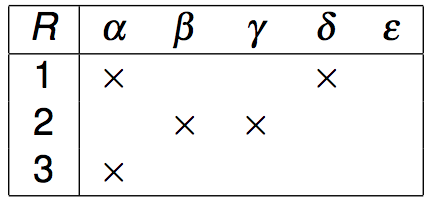
\includegraphics[scale=0.5]{images/1/RelationTable}
\end{center}

Tedy je-li $\langle x, y \rangle \in R$, je v průsečíku řádku $x$ a sloupce $y$ symbol $\times$, jinak tam není nic.

\subsubsection{Maticí}
Matice typu $m \times n$ je obdélníkové schéma o $m$ řádcích a $n$ sloupcích, ve kterém se na každém místě odpovídajícím nějakému řádku a nějakému sloupci nachází nějaká (nejčastěji číselná) hodnota. Označme tuto matici $M$, pro každé $i \in \{1, \dots,m\}$ a $j \in \{1,\dots,n\}$  Nechť $R$ je relace mezi množinami $X = \{x_1,\dots,x_m\}$ a $Y = \{y_1, \dots, y_n\}$. Potom relaci $R$ reprezentujeme maticí tak, že pokud:
$$\langle x_i,y_j\rangle \in R \text{ pak } m_{ij} = 1$$ 
$$\langle x_i,y_j\rangle \not\in R \text{ pak } m_{ij} = 0$$ 
Tuto matici nazveme \textbf{matice relace} R a značíme ji $M_R$. Matice $M_R$ relace $R = \{ \langle 1, \alpha \rangle, \langle 2, \gamma \rangle, \langle 1, \delta \rangle, \langle 2, \beta \rangle, \langle 3, \alpha \rangle\}$ mezi množinami \\$X = \{1,2,3\}$ a $Y = \{\alpha, \beta, \gamma, \delta, \epsilon\}$ bude vypadat  následovně.

\begin{displaymath}
{\bf M_R} =
\left( \begin{array}{ccccc}
1 & 0 & 0 & 1 & 0 \\
0 & 1 & 1 & 0 & 0 \\
1 & 0 & 0 & 0 & 0 \\
\end{array} \right)
\end{displaymath}

Nevýhodou této metody je její paměťová složitost. Pokud budeme mít matici $1000 \times 1000$, tak musíme v paměti uchovat milión prvků a pokud z nich bude jen 3000 rovno 1 potom zbytek uchováváme zbytečně protože víme, že na ostatních pozicích musí být 0.

Pro binární relace můžeme zavést operace, které odpovídají operacím s relacemi. Mějme binární matice $M,N$ typu $m \times n$ a matici $K$ typu $n \times k$. Definujeme následující operace:
\begin{itemize}
	\item[] $M \vee N = P, \qquad p_{ij} = max\{m_{ij}, n_{ij}\};$
	\item[] $M \wedge N = P, \qquad min\{m_{ij}, n_{ij}\};$
	\item[] $M - N = P, \qquad max\{0, m_{ij} - n_{ij}\};$
	\item[] $M \cdot K = P, \qquad max\{m_{ij} \cdot k_{ij}; I = 1, \dots ,n\};$
	\item[] $M^T, \qquad m^T_{ij} = m_{ji}$
\end{itemize}

\subsubsection{Grafem}
Grafy představují další způsob reprezentace binárních relací, který je názorný. Graf binární relace $R$ na množině $X$ dostaneme tak, že každý prvek $x \in X$ znázorníme v rovině jako kroužek s označením daného prvku. Pokud $\langle x,y \rangle \in R$, nakreslíme z uzlu $x$ do uzlu $y$ orientovanou hranu.

\begin{center}
	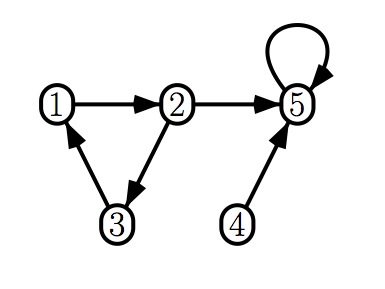
\includegraphics[scale=0.6]{images/1/RelationGraph}
\end{center}

\subsubsection{Seznamem seznamů}
Další způsob reprezentace pro uložení binární relace $R$ na množině $X$ (pro uložení binární relace v paměti počítače) je reprezentace seznamem seznamů. Tuto reprezentaci tvoří hlavní (spojový) seznam, ve kterém jsou uloženy všechny prvky množiny $X$. Z každého prcku $x \in X$ hlavního seznamu vede seznam obsahující právě ty $y \in X$, pro které platí $\langle x, y \rangle \in R$. Mějme relaci $R = \{\langle a, b\rangle,\langle a, d\rangle,\langle c, a\rangle,\langle b, d\rangle\}$ na množině $X = \{a,b,c,d\}$ potom reprezentace seznamem seznamů vypadá následovně.

\begin{center}
	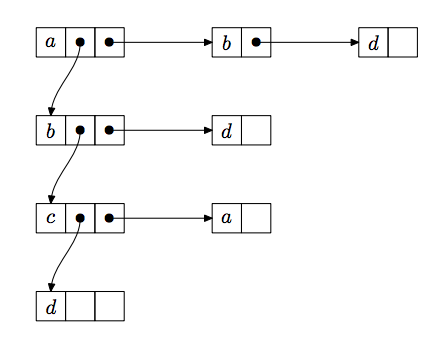
\includegraphics[scale=0.6]{images/1/RelationList}
\end{center}

\subsection{Zobrazení (funkce)}
Zobrazení (funkce) je matematickým protějškem běžně používaného pojmu přiřazení.

\begin{definition}
	Relace R mezi X a Y se nazývá zobrazení (funkce) množiny X do množiny Y, právě když pro každé $x \in X$ existuje právě jedni $y \in Y$ tak že $\langle x, y \rangle \in R$.
\end{definition}

\begin{definition}
	Zobrazení $f : X \rightarrow Y$ se nazývá
	\begin{itemize}
		\item[a)] \textbf{prosté (injektivní)}, právě když pro každé $x_1,x_2 \in X$, pro $x_1 \not= x_2$ plyne $f(x_1) \not= f(x_2)$,
		\item[b)] \textbf{surjektivní} nebo-li zobrazení X \textbf{na} Y, právě když pro každé $y \in Y$ existuje $x \in X$ tak, že  $f(x) = y$,
		\item[c)] \textbf{vzájemně jednoznačné (bijektivní)}, právě když je prosté a na (je tedy injektivní a současně surjektivní).
	\end{itemize}
\end{definition}

\begin{sentence}
	Pro zobrazení $f : X \rightarrow Y, g : Y \rightarrow Z$ platí
	\begin{itemize}
		\item[a)] $f \circ g$ je zobrazení,
		\item[b)] jsou-li f,g injekce, je $f \circ g$ injekce,
		\item[c)] jsou-li f,g surjekce, je $f \circ g$ surjekce.
	\end{itemize}
\end{sentence}

\subsubsection{Poznámka k nekonečným množinám}
\begin{definition}
	Množina A se nazývá \textbf{spočetná} , právě když existuje bijekce $f : A \rightarrow \mathbb{N}$. Množina se nazývá \textbf{nespočetná}, právě když je nekonečná a není spočetná.
\end{definition}

\subsection{Binární relace na množině}
Binární relace na množině jsou matematickým protějškem vztahů mezi dvěma prvky množiny například: \uv{$x$ je menší než $y$}. Speciálními relacemi jsou \textbf{prázdná relace $\emptyset$, relace identity} $\omega_X = \{ \langle x, x \rangle \ | \ x \in X \}$, a \textbf{kartézský čtverec} $\tau_X = X \times X$.

\begin{definition}
Nechť $R$ je binární relace na $X$. Řekněme že $R$ je
\begin{itemize}
	\item \textbf{reflexivní}, pokud pro každé $x \in X$ platí $\langle x, x \rangle \in R$
	\item \textbf{symetrická}, pokud pro každé $x,y \in X$ platí $\langle x, y \rangle \in R \Rightarrow \langle y, x \rangle \in R$
	\item \textbf{antisymetrická}, pokud pro každé $x,y \in X$ platí \\$(\langle x, y \rangle \in R \wedge \langle y, x \rangle \in R) \Rightarrow x = y$
	\item \textbf{tranzitivní}, pokud pro každé $x,y,z \in X$ platí \\$(\langle x, y \rangle \in R \wedge \langle y, z \rangle \in R) \Rightarrow \langle x, z \rangle \in R$
	\item \textbf{irreflexivní}, pokud pro každé $x \in X$ platí $\langle x,x \rangle \not\in R$
	\item \textbf{asymetrická}, pokud pro každé $x,y \in X$ platí $\langle x, y \rangle \in R \Rightarrow \langle y, x \rangle \not\in R$
	\item \textbf{úplná}, pokud pro každé $x,y \in X$ platí $\langle x, y \rangle \in R \vee \langle y, x \rangle \in R$ 
\end{itemize}
\end{definition}

Relace $R$ je \textbf{(relace) ekvivalence}, jestliže je reflexivní, symetrická, a tranzitivní. Relace $R$ je \textbf{(relace) uspořádání}, jestliže je reflexivní, anti\-symetrická a tranzitivní.

\paragraph{Reflexivita} relace $R$ vyjadřuje, že každý prvek $x \in X$ je v relace \uv{sám se sebou}. V matici takovou relaci poznáme že má na diagonále samé 1, v orientovaném grafu je u každého uzlu smyčka.

\paragraph{Symetrie} relace $R$ vyjadřuje, že $\langle x, y \rangle \in R$ právě když  $\langle y, x \rangle \in R$ Tedy relace $R$ je symetrická pokud pro $\forall x,y \in X$ máme buď současně $\langle x, y \rangle \in R$ a  $\langle y, x \rangle \in R$, nebo současně  $\langle x, y \rangle \not\in R$ a  $\langle y, x \rangle \not\in R$. Symetrickou relaci v matici $M_R$ poznáme tak, že je symetrická podle hlavní podle hlavní diagonály. V grafu se tato relace pozná tak že pokud vede orientovaná hrana z $x$ do $y$ pak musí vést i z $y$ do $x$, nebo z $x$ do $y$ nevede žádná hrana.

\paragraph{Antisymetrie} relace $R$ vyjadřuje,že pro každé dav různé prvky $x,y \in X$ neplatí současně $\langle x, y \rangle \in R$ a  $\langle y, x \rangle \in R$. V matici $M_R$ poznáme antisymetrii tak, že dvě různá pole, která jsou souměrná podle diagonály neobsahují dvě jedničky. V grafu se antisymetrie projevuje tak, že meze dvěma různými vrcholy $x,y$ je buď jedna hrana nebo žádná.

\paragraph{Tranzitivita} relace $R$ vyjadřuje, že pro pokud $\langle x, y \rangle \in R$ a pokud $\langle y, z \rangle \in R$, pak také $\langle y, z \rangle \in R$. V grafu je tranzitivita projevuje tak, že pokud vede hrana z $x$ do $y$ a zároveň z $y$ do $z$ potom také $x$ do $z$.

\paragraph{Irreflexivita} relace $R$  vyjadřuje, že žádný prvek $x \in X$ není v relaci \uv{sám se sebou}.
\paragraph{Asymetrie} relace $R$  vyjadřuje, že do $R$ nepadnou $\langle x, y \rangle$ a  $\langle y, x \rangle$ současně.
\paragraph{Úplnost} relace $R$  vyjadřuje, že aspoň jedna z dvojic $\langle x, y \rangle$, $\langle y, x \rangle$ padne do $R$.

\subsection{Uzávěry relací}
Ke každé binární relaci můžeme stanovit její reflexivní, symetrický a tranzitivní uzávěr, to je nejmenší reflexivní, symetrickou a tranzitivní relaci na dané množině, která obsahuje výchozí relaci.

\begin{sentence}
	Nechť R je binární relace na X. Pak
	\begin{itemize}
		\item Ref(R) = $R \cup \omega_X$
		\item Sym(R) = $R \cup R^{-1}$
		\item Tra(R) = $\bigcup^\infty_{n=1} R^n$, kde $R^1 = R$ a $R^n = R \circ R^{n-1}$
	\end{itemize}
\end{sentence}

\subsection{Ekvivalence}
Je binární relace, kterou lze interpretovat jako matematický protějšek nerozlišitelnosti. Pro ekvivalenci $E$ na množině $X$ definujeme pro každý $x \in X$ množinu $[x]_E = \{ y \in X \ | \ \langle x, y \rangle \in E\} $
, kterou nazýváme \textbf{třída ekvivalence prvku} x. Zřejmě $[x]_E$ obsahuje právě ty prvky z $X$, které nelze od $x$ rozlišit ekvivalencí $E$.

\subsection{Rozklad}
Rozklad na množině je matematický protějšek shluků nerozlišitelných prvků. Rozklad na $X$ je \textbf{disjuktní pokrytí} $X$.

\begin{definition}
	Nechť $X \not= \emptyset$. Systém množin $\sqcap \subseteq 2^X$ splňující
	\begin{enumerate}
		\item $Y \not= \emptyset$ pro každou $Y \in \sqcap$,
		\item pro každé $Y_1,Y_2 \in \sqcap$ platí: pokud $Y_1 \cap Y_1 \not= \emptyset$, pak $Y_1 = Y_2$,
		\item $\bigcup\sqcap = X$,
	\end{enumerate}
	se nazývá \textbf{rozklad na množině} X. Množiny $Y \in \sqcap$ nazýváme \textbf{třídy rozkladu} $\sqcap$. Pro prvek $x \in X$ označíme $[x]_\sqcap$ tu třídu rozkladu $\sqcap$, která obsahuje x. 
\end{definition} 
Na množině $X$ existuji dva mezní rozklady.Prvním z nic je rozklad $\sqcap$, kde $[x]_\sqcap = \{x\}$ pro každé $x \in X$, tj všechny třídy rozkladu $\sqcap$ jsou jednoprvkové. Druhým mezním případem je rozklad $\sqcap = \{X\}$, tj. $\sqcap$ obsahuje jedinou třídu, která je rovna celé $X$, tedy $[x]_\sqcap = X$ pro každé $x \in X$.

\begin{sentence}
	Nechť $\sqcap$ je rozklad na X. Pak binární relace $E_\sqcap$ na X definovaná $\langle x,y \rangle \in E_\sqcap$, právě když $[x]_\sqcap = [y]_\sqcap$ je ekvivalence.
\end{sentence}

Kromě ekvivalencí a rozkladů existují další přirozené pohledy na to \uv{jak zjednodušit nazírání} na výchozí množinu. Jedním z nich je \textbf{surjektivní zobrazení}. Pokud je zobrazení $f : X \rightarrow Y$ surjektivní, pak lez chápat obraz $f(x)$ prvku $x$ jako vyjádření \uv{prvek $x$ nahradíme prvkem $f(x)$}. Ukážeme, že surjektivní zobrazení a ekvivalence mají zvláštní vztah. Pro zobrazení $f : X \rightarrow Y$ definujeme binární relaci $E_f$ na $X$ předpisem $$\langle x , y \rangle \in E_f \qquad \text{právě když} \qquad f(x) = f(y)$$
Zřejmě $E_f$ je ekvivalence, tzv. \textbf{ekvivalence indukovaná zobrazením} $f$.

\subsection{Uspořádání}
Uspořádání je v informatice zcela zásadní ačkoliv si to někdy neuvědomujeme, Mezi základní každého informatika patří znalost problému třídění a typických třídicích algoritmů. Problém třídění jako takový však de facto nemá smysl uvažovat pokud bychom na množině klíčů, podle kterých třídíme, nezavedli nějakou smysluplnou relaci uspořádání -- obvykle ji však chápeme jako \uv{určenou daným kontextem} a explicitně ji nezdůrazňujeme. Uspořádání množin může výrazně zvýšit efektivitu některých algoritmů, například vyhledávání.

\begin{definition}
	Reflexivní, antisymetrická a tranzitivní binární relace R na X se nazývá \textbf{uspořádání}. Úplné uspořádání se nazývá \textbf{lineární uspořádání} neboli \textbf{řetězec}. Pokud je R uspořádání na X, pak se $\langle X, R \rangle$ nazývá \textbf{upořádáná množina}.
\end{definition}

Relace uspořádání na $X$ obvykle značíme $\leq$ v souladu s intuitivním chápáním uspořádání a místo $\langle x ,y \rangle \in \ \leq$. Zdůrazněme ale, že označení $\leq$ v tuto chvíli nemá (obecně) nic společného se srovnáváním čísel, na které jsme zvyklí. Uspořádání pořád ještě není formálním protějškem \uv{upořádání} na které jsme zvyklí při porovnávání čísel. Je-li $\langle X, \leq \rangle$ uspořádaná množina, pak mohou  existovat $x,y \in X$ ,pro které neplatí $x \leq y$ ani $y \leq x$ (definice to nevylučuje). V tom případě říkáme, že prvky jsou \textbf{nesrovnatelné} což někdy značíme $x\ \| \ y$. V opačném případě prvky nazýváme \textbf{srovnatelné}. Je-li $\leq$ lineární uspořádání na $X$, pak je $\leq$ úplná relace, což znamená, že každé prvky jsou srovnatelné. Lineární uspořádání lze tedy chápat jako matematický protějšek \uv{tradičního srovnávání čísel}. Každá relace identity $\omega_X$ je uspořádání které nazýváme \textbf{antiřetězec}  

\begin{sentence}
	Princip duality. Nechť $\leq$ je uspořádání na $X$. Pak $\leq^{-1}$ je uspořádání na $X$, které označujeme $\geq$.
\end{sentence}

Konečné uspořádání $\leq$ na $X$ je relace, mžeme ji tedy reprezentovat binární maticí nebo příslušným orientovaným grafem. Díky speciálním vlastnostem konečných uspořádání je však můžeme znázorňovat mnohem přehledněji pomocí speciálních diagramů. Ke každému uspořádání $\leq$ na $X$ lze uvažovat odvozenou relaci $\prec$ definovanou předpisem
$$x \prec y, \text{ právě když } x \leq y \text{ a } \forall z \in X \text{ platí: }$$
$$\text{pokud} y \leq z \leq y, \text{ pak } z \in \{ x, y\}$$



Relaci $\prec$ nazýváme pokrytí příslušné $\leq$ , a výraz $x \prec y$ čteme \uv{x je pokryt y} nebo \uv{x pokrývá y}. Na relaci pokrytí je založena jedna z metod jak znázornit konečnou uspořádanou množinu, tak zvané \textbf{Hasseovy diagramy} uspořádaných množin.

\begin{center}
	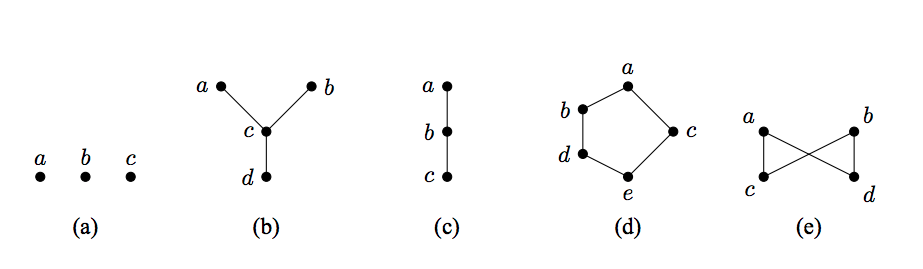
\includegraphics[scale=0.9]{images/1/HasseDiagrams}
\end{center}

\begin{definition}
	Nechť $\langle X, \leq \rangle$ je uspořádaná množina. Prvek $x \in X$ se nazývá
	\begin{itemize}
		\item \textbf{minimální}, jestliže $\forall y \in X$ platí: pokud $y \leq x$, pak $x = y$,
		\item \textbf{nejmenší}, jestliže $x \leq y$ pro každá $y \in X$,
		\item \textbf{maximální}, jestliže $\forall y \in X$ platí: pokud $y \geq x$ pak $x = y$,
		\item \textbf{nejmenší}, jestliže $x \geq y$ pro každý $y \in X$.
	\end{itemize}
\end{definition}

\begin{sentence}
	Nechť $\langle X, \leq \rangle$ je uspořádaná množina. Pak platí
	\begin{enumerate}
		\item v $\langle X, \leq \rangle$ existuje nejvýše jeden největší a nejvýše jeden nejmenší prvek;
		\item je-li $x \in X$ největší (nejmenší) prvek, pak je také maximální (minimální);
		\item pokud je $\leq$ lineární uspořádání, pak je $x \in X$ největší (nejmenší) prvek, právě když je maximální (minimální).
	\end{enumerate}
\end{sentence}

\begin{definition}
	Nechť $\langle X, \leq \rangle$ je uspořádaná množina a nechť $Y \subseteq X$. Definujeme množiny
	$$L(Y) = \{ x \in X \ | \ x \leq y \text{ platí pro každé } y \in Y\}$$
	$$U(Y) =  \{ x \in X \ | \ x \geq y \text{ platí pro každé } y \in Y\}$$
	L(Y) se nazývá \textbf{dolní kužel množiny} Y v  $\langle X, \leq \rangle$. U(Y) se nazývá \textbf{horní kužel množiny} Y v  $\langle X, \leq \rangle$.
\end{definition}

Jinými slovy dolní kužel množiny $Y$ v  $\langle X, \leq \rangle$ obsahuje tedy právě ty prvky z $X$, které jsou menší nebo rovny všem prvkům obsaženým v $Y$, analogicky pro horní kužel.

\begin{definition}
	Nechť  $\langle X, \leq \rangle$ je uspořádaná množina a nechť $Y \subseteq X$. Pokud má $L(Y)$ největší prvek, pak se nazývá \textbf{infimum} Y a označuje se $inf(Y)$. Pokud má $U(Y)$ nejmenší prvek, pak se nazývá \textbf{supremum} Y a označuje se $sup(Y)$.
\end{definition}

\begin{definition}
	Nechť  $\langle X, \leq \rangle$ je uspořádaná množina. Pokud pro každé $x,y \in X$ existuje $inf(x,y)$, pak  $\langle X, \leq \rangle$ nazveme \textbf{průsekový polosvaz}. Pokud pro každé $x,y \in X$ existuje $sup(x,y)$ pak  $\langle X, \leq \rangle$ nazveme \textbf{spojový polosvaz}. Je-li  $\langle X, \leq \rangle$ průsekový i spojový polosvaz, pak  $\langle X, \leq \rangle$ nazveme \textbf{svaz}.
\end{definition}

\end{document}
